\documentclass[11pt,a4paper]{article}
\usepackage{fontspec}
\setmainfont{TeX Gyre Pagella}
\newfontfamily\headfont{Inter}[UprightFont=*-ExtraBold,BoldFont=*-ExtraBold,Extension=.otf,Path=/usr/share/fonts/opentype/inter/]
\usepackage[a4paper,margin=2.3cm]{geometry}
\usepackage{graphicx,booktabs,float,caption,array,xcolor,longtable}
\usepackage{xurl}
\usepackage[hidelinks]{hyperref}
\usepackage{titlesec}
\usepackage[round]{natbib}
\usepackage{setspace}
\setstretch{1.05}
\renewcommand{\topfraction}{0.9}
\renewcommand{\bottomfraction}{0.8}
\renewcommand{\textfraction}{0.1}
\renewcommand{\floatpagefraction}{0.75}
\setlength{\parindent}{0pt}
\setlength{\parskip}{0.55em}
\titleformat{\section}{\headfont\Large}{\thesection}{0.8em}{}
\titleformat{\subsection}{\headfont\large}{\thesubsection}{0.8em}{}
\captionsetup{font=small,labelfont=bf}
\urlstyle{same}
\hypersetup{pdftitle={Named for a Place, Living Somewhere Else?},pdfauthor={Tristan Hotham}}

\begin{document}
\begin{center}
{\Large\bfseries Named for a Place, Living Somewhere Else?\par}
\vspace{0.4em}
{\large Species named after places, tested against where GBIF records them\par}
\vspace{1.2em}
{\large Tristan Hotham\par}
\vspace{0.3em}
{\small Independent researcher\\
ORCID: 0000-0003-4931-9349\\
DOI: https://doi.org/10.5281/zenodo.24058123\par}
\vspace{0.8em}
2026
\end{center}

\begin{quote}
\small
\begin{center}\textbf{Abstract}\end{center}
Many species are named after a place, usually the place their type specimen came from. I test whether they live there, using two sources. First, Wikidata links 2,901 species and subspecies (after merging duplicate items) to a place with coordinates through ``named after''. Matching them to the Global Biodiversity Information Facility (GBIF) and counting occurrence records by country, 1,210 plants, animals and fungi have enough records to test: 98\% are recorded in the country of their namesake, 88\% have most of their records there, and 70\% have no records elsewhere. Among 38 microbes and viruses the share recorded at home falls to 66\%, and among fungi to 81\%. After a hand check of every case, which found that 24 of 53 apparent misses were errors in the data (duplicate items, synonym keys, regions pinned on one country and wrong links), 29 plants, animals and fungi with at least 5 records have none in their namesake country. They include classic misnomers such as the coco de mer \textit{Lodoicea maldivica}, recorded in the Seychelles, and the Javan banded pitta \textit{Pitta guajana}, but most are gaps in the records: fossils, marine species and taxa recorded just across a border. Second, for 202 Latin place adjectives (\textit{anglica}, \textit{japonica} and so on) covering 61,815 Wikidata taxa, a stratified sample suggests that about 91\% are recorded in their place; the British and Irish epithets, checked in full, score lower (81\%).

\textbf{Keywords:} biological nomenclature; toponyms; specific epithets; GBIF; Wikidata; species distributions; misnomers
\end{quote}

\section{Introduction}
Place names are among the commonest sources of scientific names. A species called \textit{japonica} or \textit{californicus}, or named in honour of a mountain or an island, normally takes its name from the locality of its type specimen, or from the region its describer thought it came from. Names, once published, are fixed by the rules of nomenclature even when they turn out to be misleading. This raises a simple question that is now possible to answer at scale: do species named after a place actually live there?

Two open sources make the test possible. Wikidata \citep{wikidata} records, for some taxa, the entity a name commemorates (property P138, ``named after''), with coordinates and a country. GBIF aggregates hundreds of millions of georeferenced occurrence records and indexes them against a taxonomic backbone \citep{gbif}. GBIF's coverage is famously uneven \citep{beck2014,meyer2016}, so this paper treats its records as evidence of presence, not of absence, and reports the misses as leads rather than facts.

\section{Data}
\textbf{Named taxa.} A Wikidata query returned every taxon with a ``named after'' link to an item with coordinates, with the item's country and type, and the taxon's GBIF key (P846). I kept species and subspecies (2,988 items), dropped 36 whose namesake is a ship or an institution rather than a place (universities, museums, research vessels), and counted once the 51 items that share a GBIF accepted taxon and a namesake with another (recombinations and old genera, such as \textit{Hydrornis guajanus} and \textit{Pitta guajana}), keeping the item on the accepted key. That leaves 2,901 taxa (2,745 species, 156 subspecies). 2,423 have a GBIF key, 175 of them through an exact match of the name to the GBIF backbone for taxa without a key in Wikidata.

\textbf{GBIF records.} For each key I retrieved from the GBIF API the number of occurrence records with coordinates, no geospatial issue and status ``present'', their counts by country (the country facet), the bounding box of the records from the density-map capabilities service (in whole degrees), and the backbone classification. 1,375 taxa have at least one such record; the median assessed taxon has 10.

\textbf{Latin epithets.} I listed 202 Latin adjectives that unambiguously denote a place (e.g. \textit{anglica}, \textit{scoticus}, \textit{hibernicum}, \textit{londinensis}, \textit{japonica}, \textit{canadensis}), grouped into 79 places, of which 12 are regions spanning several countries (the Caucasus, the Himalaya, Patagonia, Arabia, Borneo and others). I dropped \textit{argentina}, which also means silvery. Wikidata holds 61,815 species and subspecies whose final epithet is one of these words, 53,257 with a GBIF key. I retrieved GBIF country counts for every British and Irish one with a key (660) and a random sample of up to 40 taxa with a key for each other adjective (7,756 in all, after counting once the few GBIF keys shared by two spellings of a name).

\section{Method}
A taxon's test countries are the countries Wikidata gives for its namesake, the country (or territory, as GBIF codes it) that contains the namesake's coordinates in Natural Earth, and the overseas territories of those countries that GBIF codes separately (French Guiana for France, Greenland for Denmark, St Helena for the United Kingdom). For continents and for regions that cross borders but that Wikidata places in one country (Africa, Europe, Asia, Macedonia, the Balkans, the Guianas, the Caucasus, Togoland, Arabia Petraea) the test countries are all those the region covers; these overrides are listed in the data. Subnational regions are tested at the level of their country, which is generous: a taxon named for Siberia passes if it is recorded anywhere in Russia. GBIF assigns a country to records in a country's waters, so marine taxa are tested like others; records on the high seas or in disputed areas carry no country and count for none, and the 9 taxa whose namesake has no country (open ocean, Antarctica) are not assessed. A taxon is \emph{recorded there} if any GBIF record is in a test country, and \emph{not there} if it has at least 5 records and none in a test country. Taxa with fewer records and none at home, or with none at all, are not assessed. GBIF counts records under a synonym's key only if they were filed under that name, so a synonym key can show presence but not absence: the 7 synonym-keyed taxa with no records at home are not assessed. The \emph{share at home} is the fraction of a taxon's records in its test countries. For taxa not recorded there, the distance from the namesake to the nearest point of the records' bounding box is a crude measure of how far off the name is. Groups follow the GBIF backbone (kingdom and class).

\textbf{Checks.} I reviewed by hand every plant, animal and fungus first found not to be recorded at home (53), a random 30 of those recorded at home, and every assessed name whose epithet does not echo its namesake's name. Of the 53 apparent misses, 5 were duplicate items, 7 rested on synonym keys, 3 were regions pinned on a single country and 9 were wrong links (45\% in all); the random sample of those at home held 3 wrong links in 30, and the full check of non-echoing names found 49, most of them links to a person honoured in the name or to a common name (the Bermuda grass \textit{Cynodon dactylon}, the Key lime \textit{Citrus} \texttimes\textit{aurantifolia}). The 58 wrong links are left out of all results; the review and the overrides are published with the data. Microbes and viruses were not reviewed.

For the epithets the test country is the one the adjective names, or every country of a multi-country region. Because the non-British sample is stratified by adjective, I report a weighted share in which each sampled taxon carries the inverse of its adjective's sampling fraction (taxa with a GBIF key for the adjective divided by taxa sampled), so that each adjective counts in proportion to its size.

\section{Results}
\subsection{Most taxa are recorded where they are named}
Of 1,210 assessed plants, animals and fungi, 98\% are recorded in their namesake's country, 88\% have most of their records there and 70\% have all of them there (Figures~\ref{fig:world} and~\ref{fig:share}). Widespread taxa naturally have a smaller share at home: among the 253 with at least 100 records, 98\% are recorded there but only 71\% have most records there.

\begin{figure}[tbp]\centering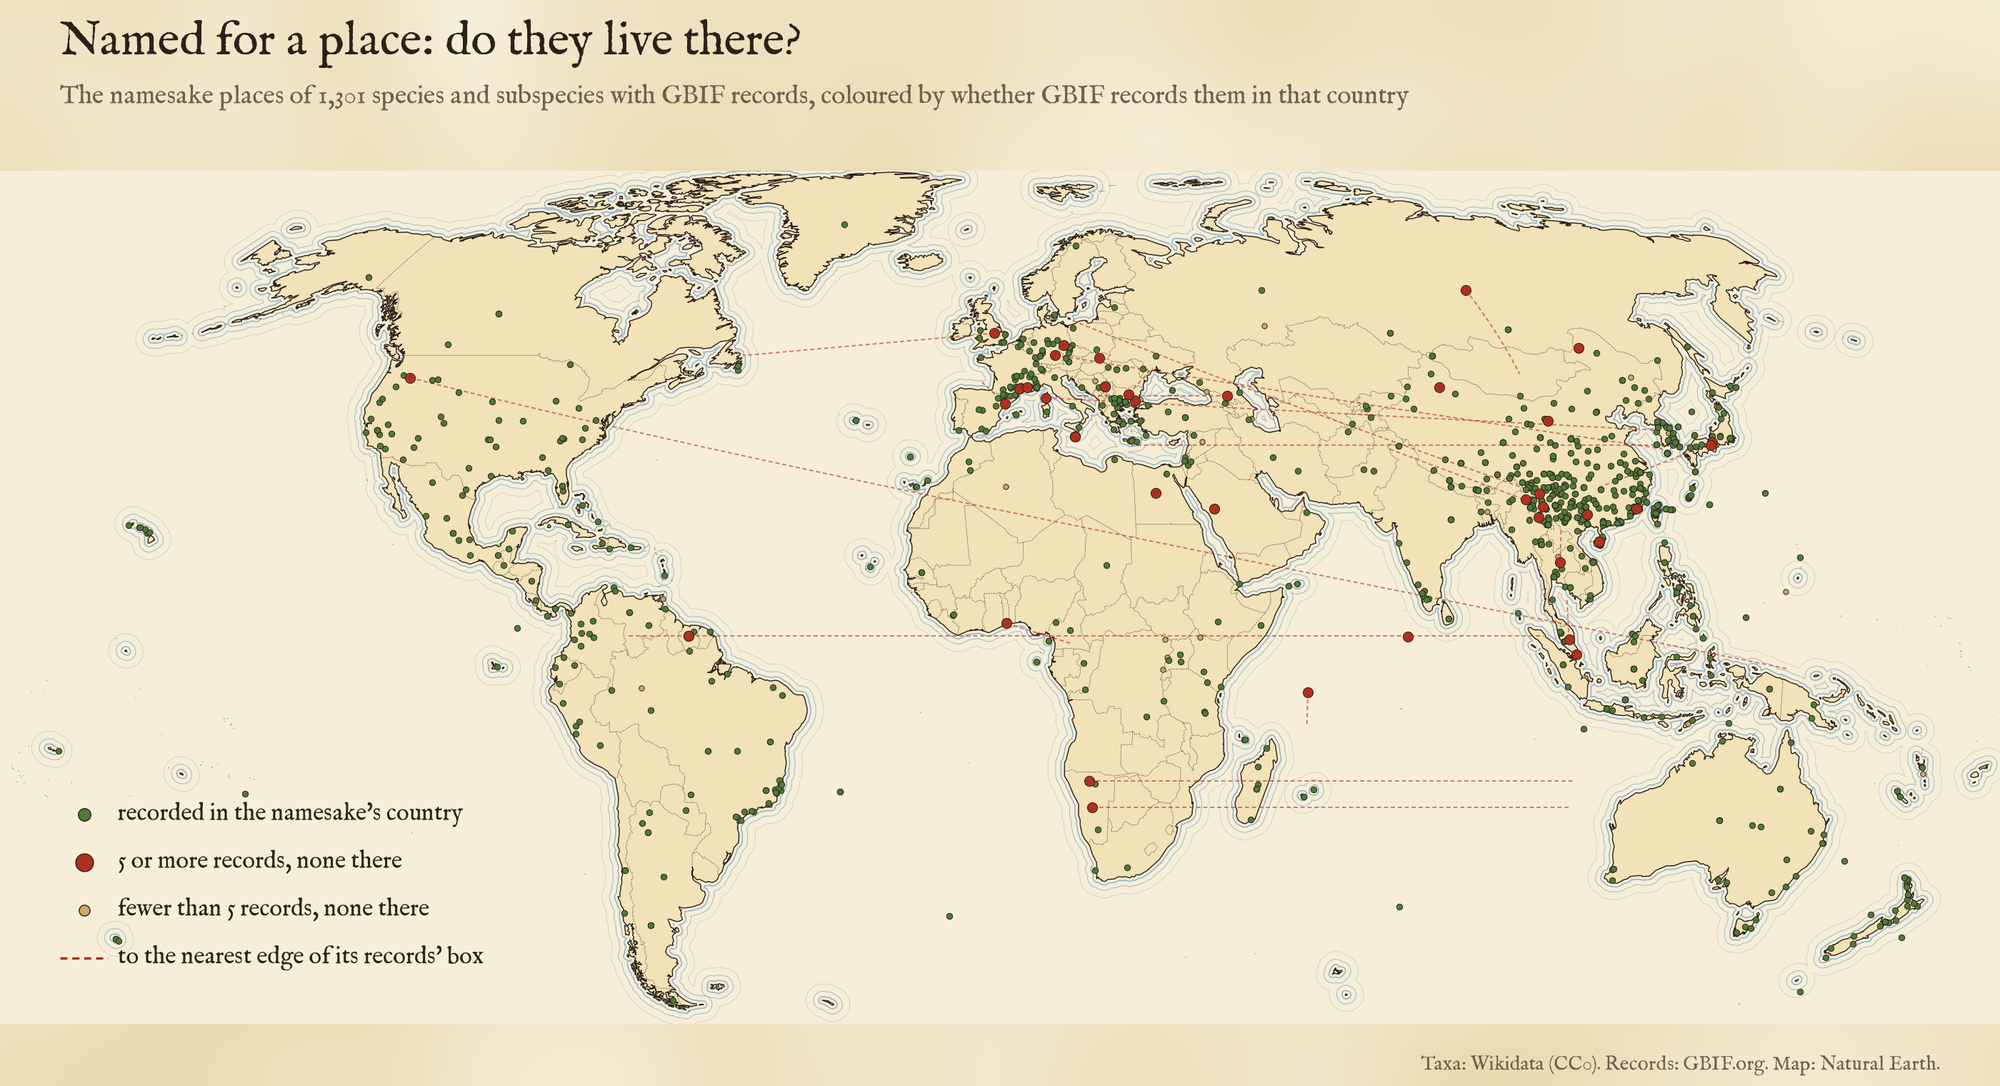
\includegraphics[width=\textwidth]{f_world.png}
\caption{Namesake places of the assessed taxa, coloured by verdict. Red lines join the namesakes of taxa not recorded there to the nearest edge of their records' bounding box.}\label{fig:world}\end{figure}
\begin{figure}[tbp]\centering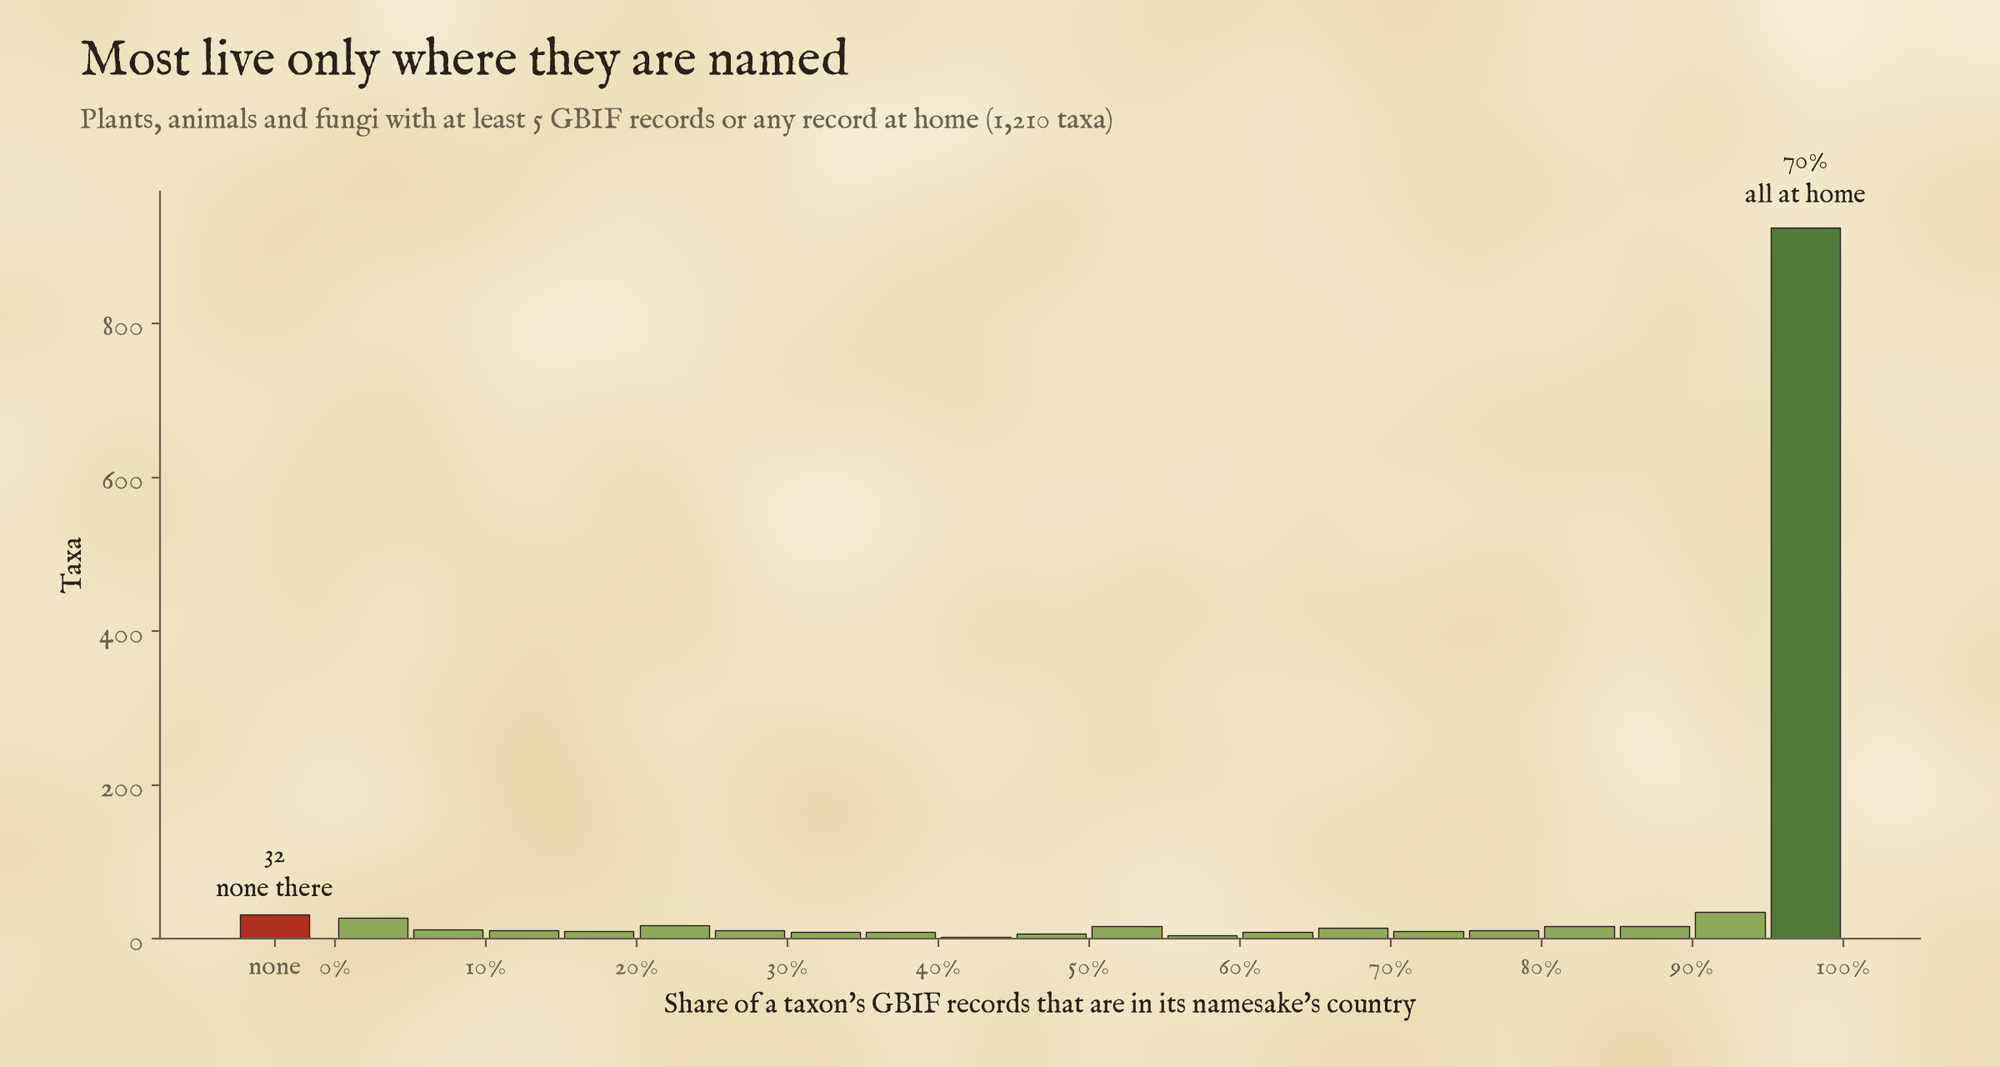
\includegraphics[width=0.85\textwidth]{f_share.png}
\caption{Share of each taxon's GBIF records that lie in its namesake's country.}\label{fig:share}\end{figure}

\subsection{Groups}
Table~\ref{tab:groups} and Figure~\ref{fig:groups} compare groups. Reptiles (98\%), insects (100\%), arachnids (98\%), plants (98\%) and amphibians (97\%) are almost always recorded at home. Birds are recorded at home in 98\% of cases but have most records there in only 69\%, reflecting dense observation of widespread birds elsewhere. Fungi (81\%) and microbes (66\%) score lowest; many microbial ``occurrences'' are culture-collection strains or environmental sequences.

\begin{table}[tbp]\centering\small\caption{Assessed taxa by group: number, share recorded in the namesake's country, share with most records there, and number not recorded there.}\label{tab:groups}\begin{tabular}{lrrrr}\toprule Group & Assessed & Recorded there & Mostly there & Not there\\\midrule
Plants & 587 & 98\% & 89\% & 9\\
Insects & 151 & 100\% & 93\% & 0\\
Other invertebrates & 98 & 96\% & 90\% & 4\\
Fish & 74 & 96\% & 89\% & 3\\
Mammals & 66 & 95\% & 82\% & 3\\
Amphibians & 59 & 97\% & 86\% & 2\\
Birds & 54 & 98\% & 69\% & 1\\
Reptiles & 48 & 98\% & 88\% & 1\\
Spiders, mites and scorpions & 47 & 98\% & 96\% & 1\\
Microbes, viruses and other & 38 & 66\% & 26\% & 13\\
Fungi and lichens & 26 & 81\% & 54\% & 5\\
\bottomrule\end{tabular}\end{table}
\begin{figure}[tbp]\centering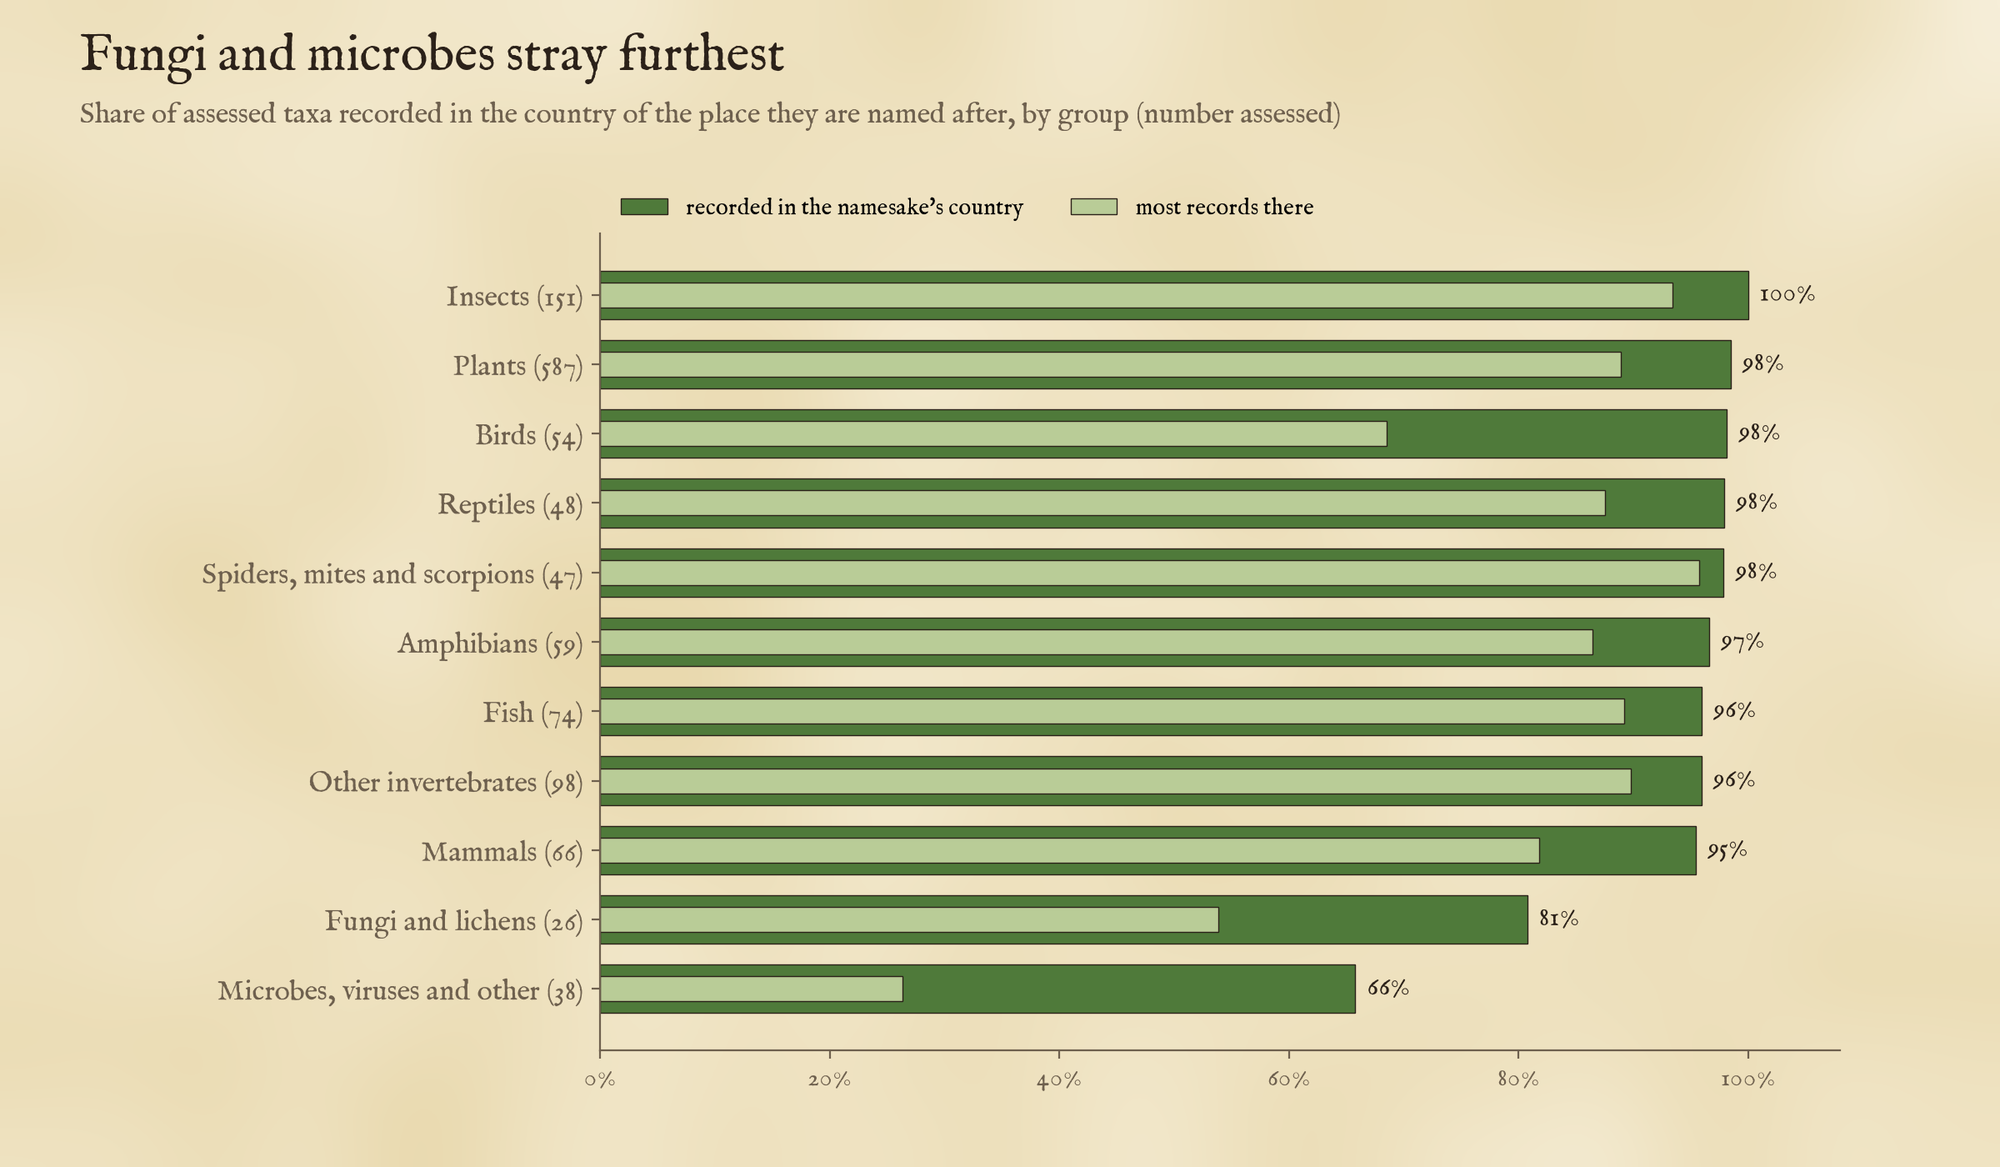
\includegraphics[width=0.85\textwidth]{f_groups.png}
\caption{Share recorded in the namesake's country, and share with most records there, by group.}\label{fig:groups}\end{figure}

\subsection{The misnamed}
After the checks, 29 plants, animals and fungi with at least 5 records have none in their namesake's country; for 9 of them the namesake still lies inside the records' bounding box, and the median distance to the box is 217 km. Table~\ref{tab:no} lists those with most records. Only 3 are clear misnomers. The coco de mer, \textit{Lodoicea maldivica}, takes its name from the Maldives, where its nuts were found washed ashore \citep{capasia}, but 292 of its 301 records are in the Seychelles. The Javan banded pitta, \textit{Pitta guajana} in the GBIF backbone (\textit{Hydrornis guajanus}), bears the name of the Guianas from Buffon's ``merle de la Guiane'', its type locality since corrected to Java \citep{ioc}; 301 of its 353 records are in Indonesia. The Central Asian salamander \textit{Ranodon sibiricus} is named for Siberia, lives in the Dzungarian Alatau, and was described from a type locality near Semipalatinsk now considered erroneous \citep{frost}.

The rest are better read as gaps in GBIF. The Guinea worm \textit{Dracunculus medinensis} is the ``little dragon from Medina'' \citep{eid2016}, from a time when it was common in Arabia; it is now near eradication and GBIF holds no Saudi records. Several are fossils whose type locality is not in GBIF: the dwarf elephant \textit{Elephas melitensis} of Malta, with 31 records from Sicily, and the Ediacaran \textit{Bradgatia linfordensis} of Charnwood Forest, recorded only from Newfoundland. Some are marine (\textit{Leucoraja melitensis}, recorded in Italian, Algerian and Tunisian waters), some sit just over a border (\textit{Verbascum adrianopolitanum}, named for Edirne and recorded in Greece and Bulgaria), and some fungi are recorded only far from home (\textit{Aspergillus egyptiacus}, 297 of 393 records in Australia). Figure~\ref{fig:misnamed} maps seven.

\begin{table}[tbp]\centering\small\caption{Plants, animals and fungi with most GBIF records and none in their namesake's country.}\label{tab:no}\begin{tabular}{llrl}\toprule Taxon & Named after & Records & Most records\\\midrule
\textit{Aspergillus egyptiacus} & Egypt & 393 & Australia 297, Oman 53\\
\textit{Pitta guajana} & Guyanas & 353 & Indonesia 301, Malaysia 34\\
\textit{Lodoicea maldivica} & Maldives & 301 & Seychelles 292, France 2\\
\textit{Ranodon sibiricus} & Siberia & 226 & Kazakhstan 220, China 6\\
\textit{Panthera gombaszoegensis} & Gombasek & 61 & Netherlands 17, Tanzania 8\\
\textit{Melicope pahangensis} & Pahang & 45 & China 35, Laos 6\\
\textit{Cordyceps ningxiaensis} & Ningxia & 40 & Sweden 22, Norway 8\\
\textit{Suillellus caucasicus} & Caucasus Mountains & 39 & France 20, Spain 7\\
\textit{Camellia indochinensis} & Mainland Southeast Asia & 33 & China 32, United States 1\\
\textit{Elephas melitensis} & Malta & 31 & Italy 31\\
\textit{Dracunculus medinensis} & Medina & 25 & Benin 17, United States 6\\
\textit{Leucoraja melitensis} & Malta & 22 & Italy 11, Algeria 4\\
\textit{Stachys serbica} & Serbia & 18 & Greece 18\\
\textit{Bachia guianensis} & Guyanas & 17 & Colombia 16, Venezuela 1\\
\textit{Bradgatia linfordensis} & Newtown Linford & 16 & Canada 16\\
\textit{Notidanus aptiensis} & Apt & 15 & United Kingdom 14, Australia 1\\
\textit{Verbascum adrianopolitanum} & Edirne & 14 & Greece 9, Bulgaria 4\\
\textit{Catatemnus togoensis} & Togoland & 10 & DR Congo 10\\
\bottomrule\end{tabular}\end{table}
\begin{figure}[tbp]\centering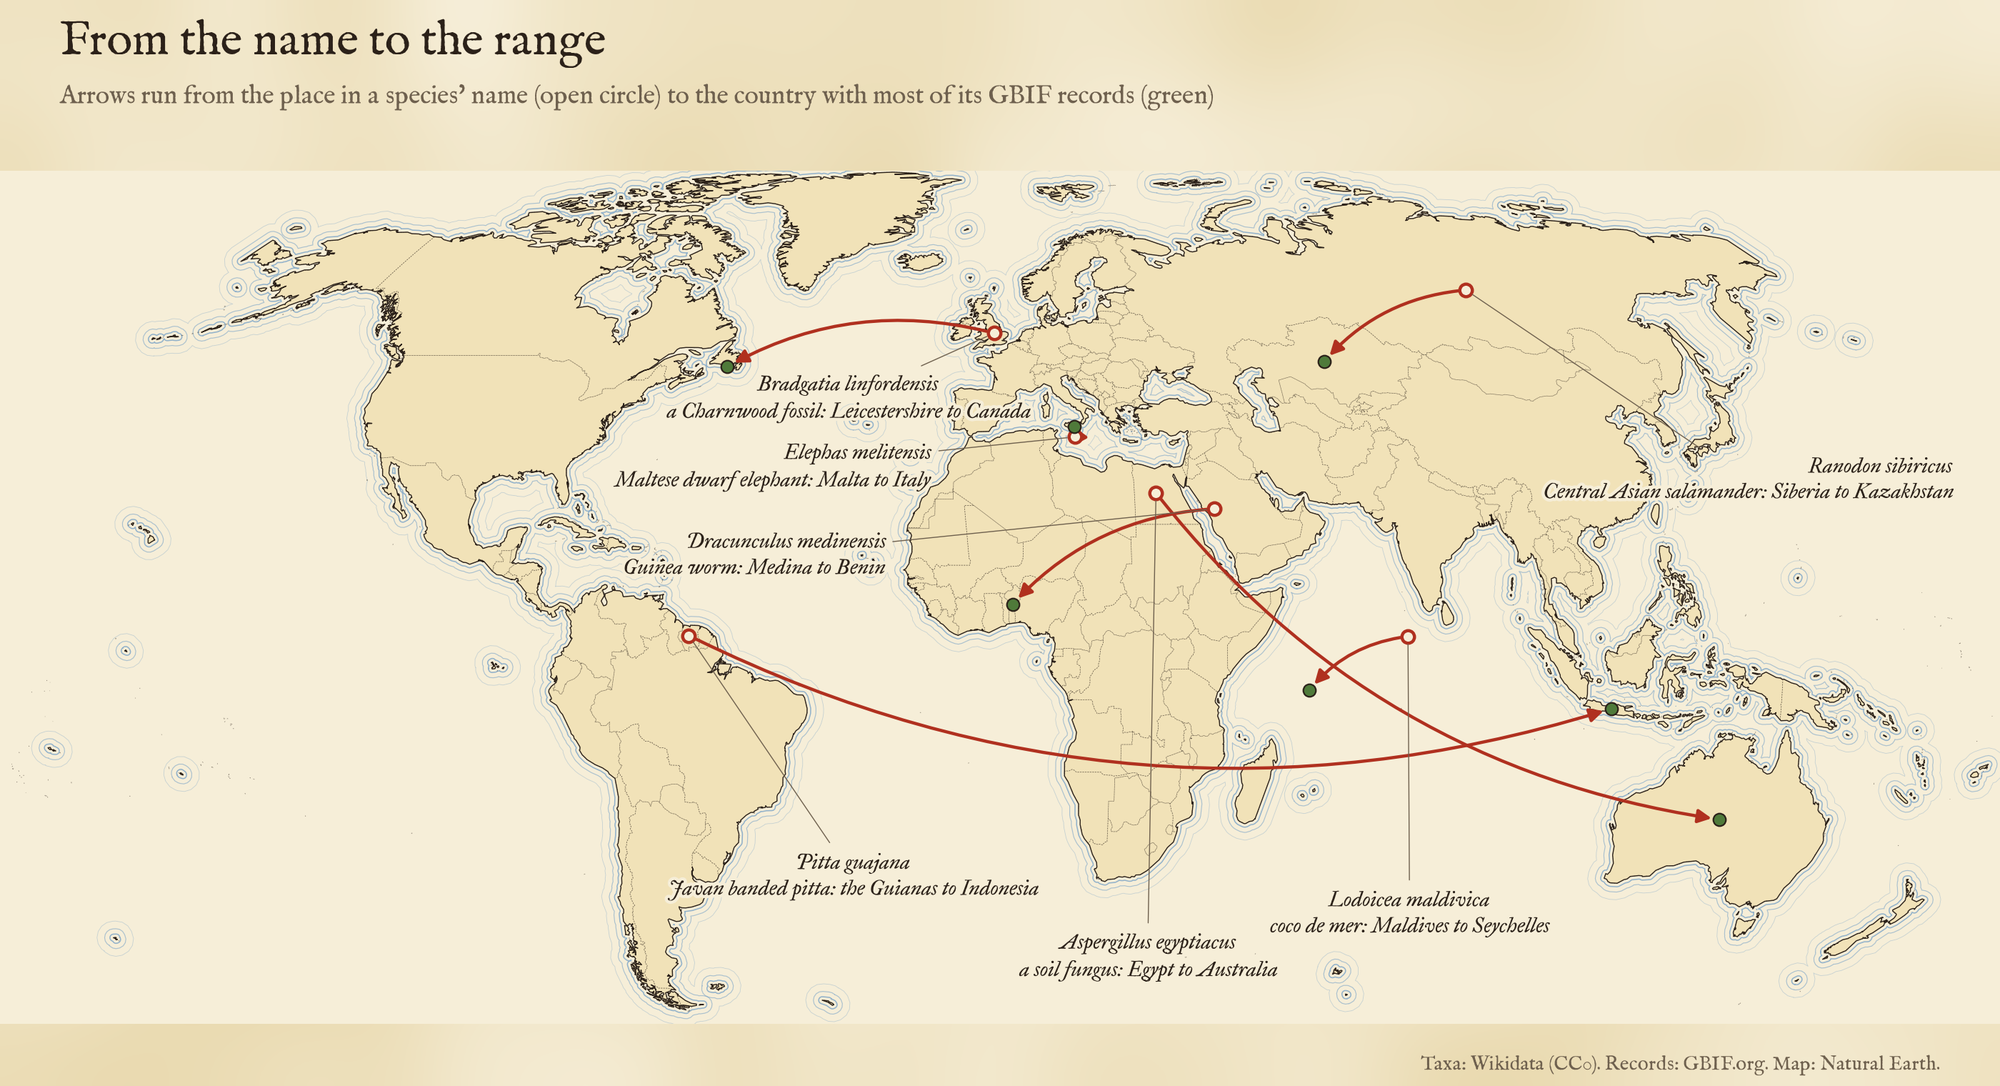
\includegraphics[width=\textwidth]{f_misnamed.png}
\caption{From namesake to range for seven taxa not recorded in their namesake's country.}\label{fig:misnamed}\end{figure}

\subsection{Latin place epithets}
Of 3,565 sampled epithet taxa with enough records, the weighted share recorded in the named place is 91\% for the non-British adjectives (unweighted 91\%). Of 69 places with at least 15 assessed taxa, 9 have every one recorded there; the lowest are Hungary (54\%), Mongolia (68\%) and Egypt (69\%) (Figure~\ref{fig:epithets}). The British and Irish adjectives, checked in full, score 81\% over 323 taxa (Figure~\ref{fig:british}), from 90\% for \textit{britannica} to 61\% for \textit{hibernica}, for which only the Republic of Ireland counts. Some misses are names that only look British: \textit{Chrysoblephus anglicus} is a South African sea bream and \textit{Urophyllum britannicum} is recorded only in Papua New Guinea. Others are recording artefacts: \textit{Potentilla anglica} subsp. \textit{anglica} has 2,154 records in Germany and France and none in Britain.

\begin{figure}[tbp]\centering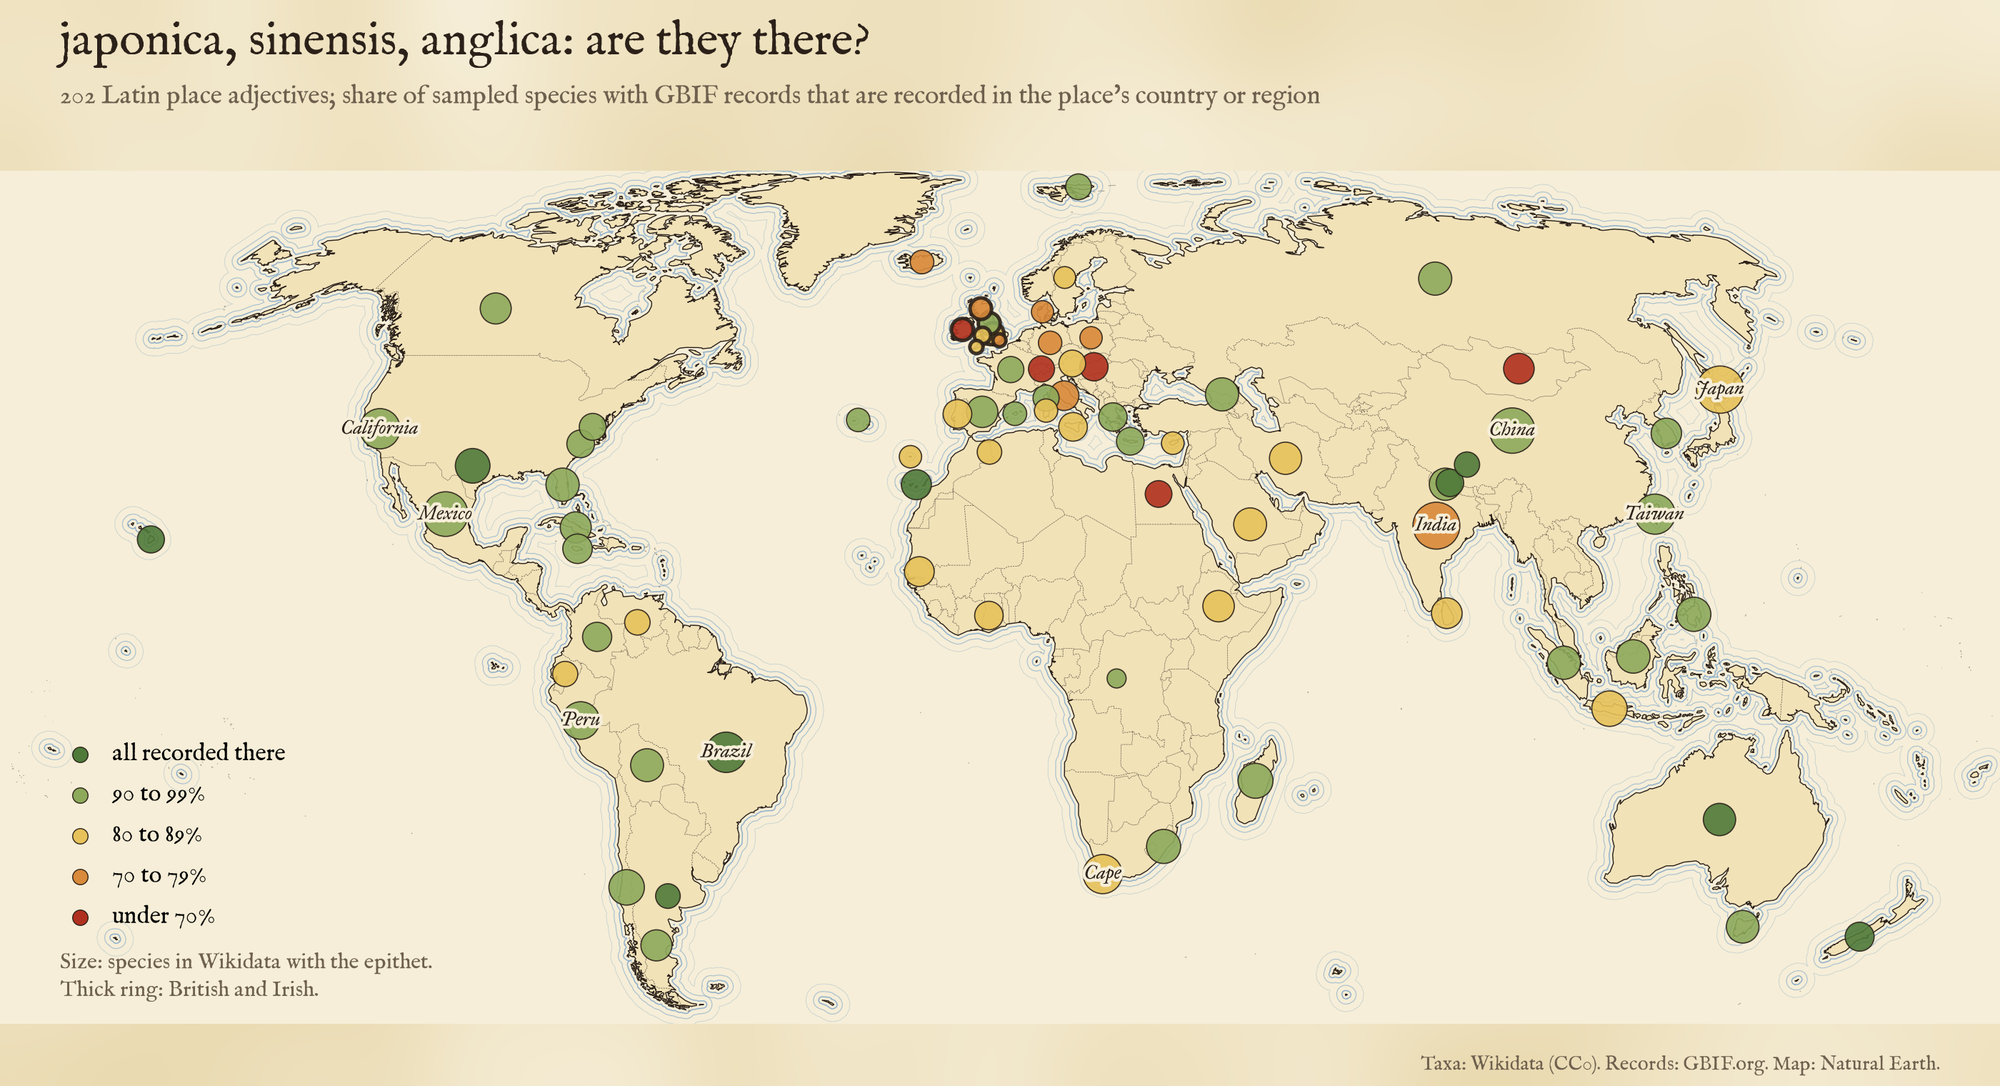
\includegraphics[width=\textwidth]{f_epithets.png}
\caption{Latin place epithets: share of sampled taxa recorded in the named country or region.}\label{fig:epithets}\end{figure}
\begin{figure}[tbp]\centering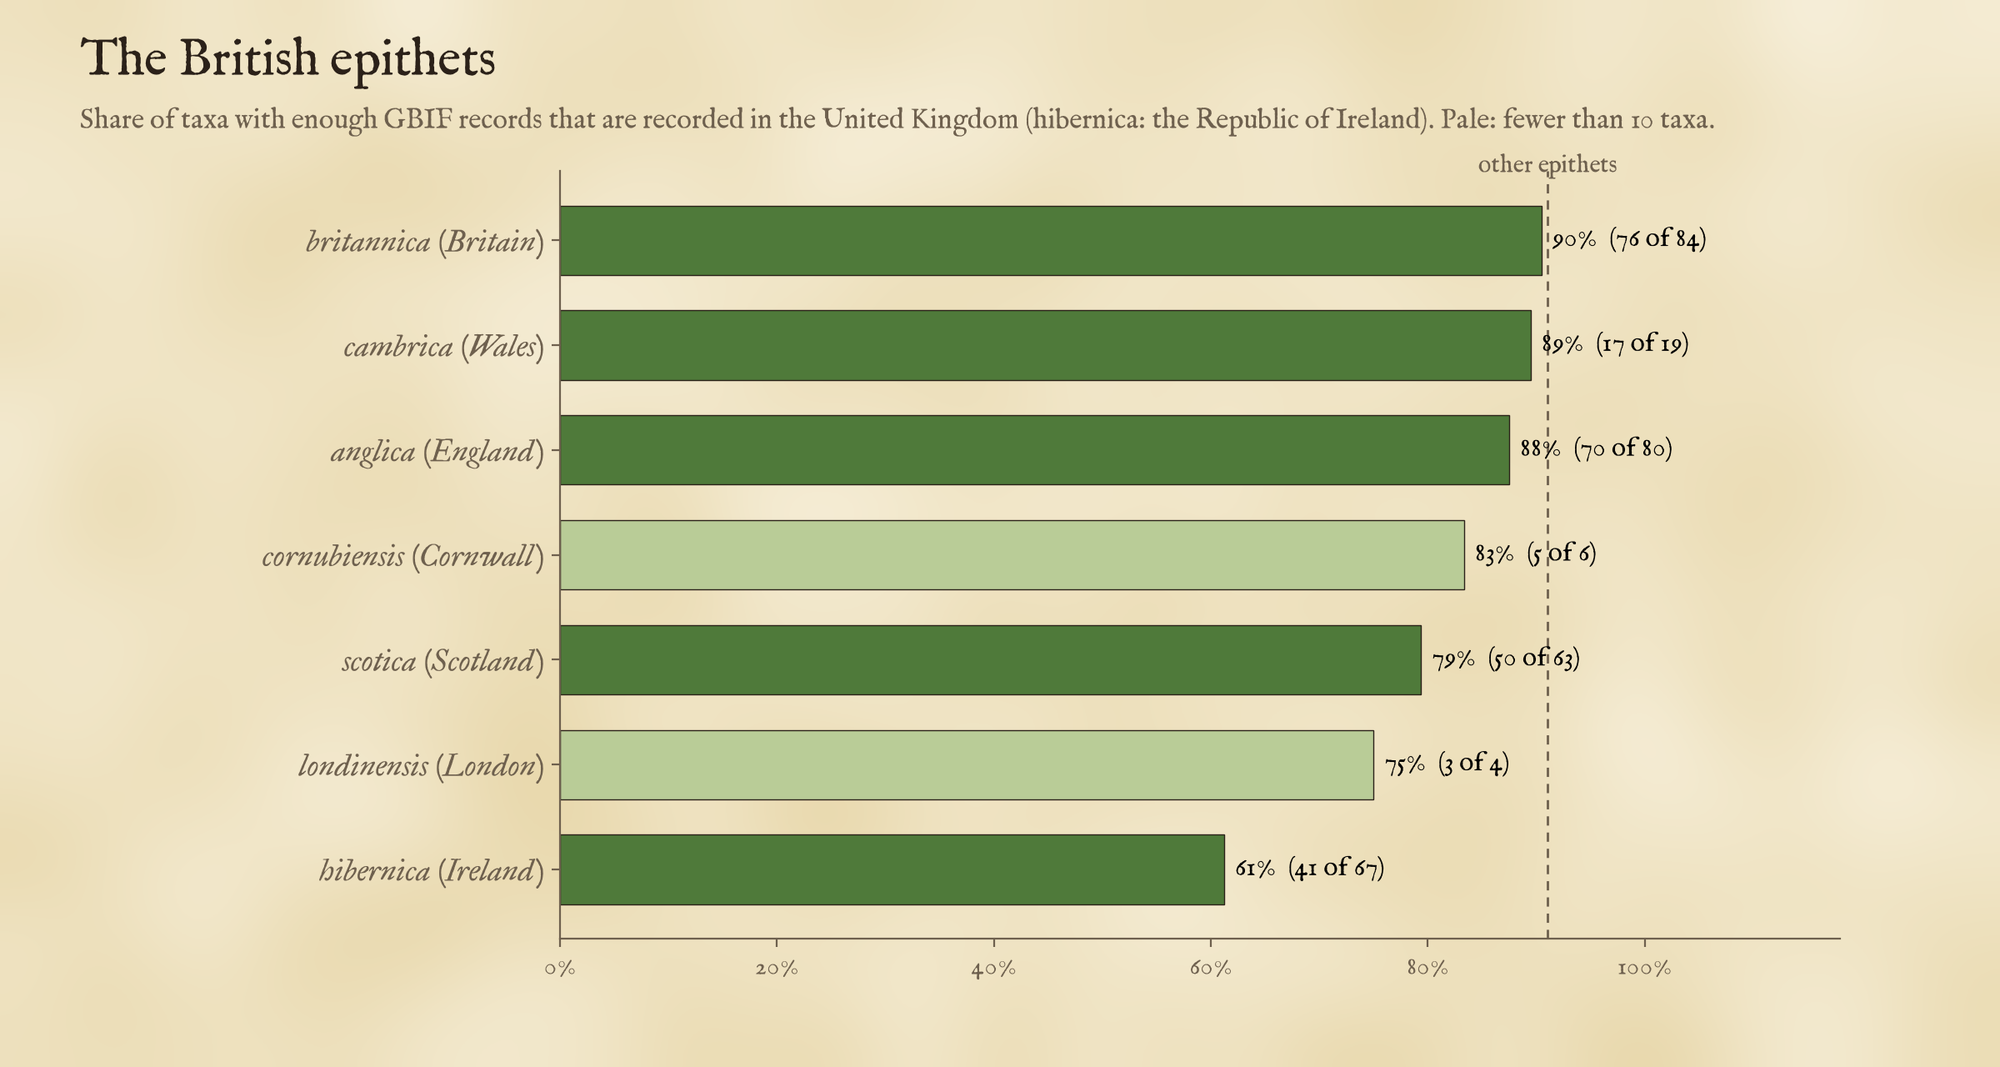
\includegraphics[width=0.85\textwidth]{f_british.png}
\caption{British and Irish epithets.}\label{fig:british}\end{figure}

\section{Limitations}\label{sec:limits}
GBIF is a record of where people have looked and shared data, not of where species live \citep{beck2014,meyer2016}. Presence in a country is easy to establish because type specimens and the material collected with them are often in GBIF; absence is weak evidence, and many taxa have too few records to test at all. Country is a coarse unit: a species named for a town may live only far from it, and the bounding boxes are inflated by single stray records, such as botanic garden plants. Records are counted under the GBIF key of the name, so records filed under a synonym, the species rather than a subspecies, or a different concept are missed. Wikidata's ``named after'' links cover a small, uneven subset of names and some are wrong; the hand checks covered every apparent miss and every assessed name that does not echo its namesake, but not the untested taxa or the microbes, and a wrong link whose epithet happens to resemble its namesake would pass. Duplicates are removed only where GBIF maps two items to the same accepted taxon; synonymy that GBIF does not record is not caught, and in the epithet layer, which has no backbone status, only items sharing a GBIF key are merged. The epithet test cannot know what an author meant, and the non-British epithet results are from a sample.

\section{Conclusion}
Most species named after a place are recorded there, and most live mostly there. The exceptions are a mixture of famous misnomers, shifting borders, wide-ranging and easily dispersed organisms, and errors in the data that links names to places. The interactive page lets anyone explore every case.

\section*{Data and code availability}
The interactive page is at \url{https://maps.tristanhotham.com/species-places/}. Derived data and code are at \url{https://github.com/Tristan-Hotham/species-places} and archived with this paper at https://doi.org/10.5281/zenodo.24058123. Text, figures and derived data are CC BY 4.0 and code MIT. Wikidata content is CC0. GBIF counts are aggregated from records published under CC0, CC BY and CC BY-NC and are cited to GBIF.org; no record-level data are redistributed.

\section*{AI statement}
I wrote the text, with drafting and editing assistance from Claude (Anthropic), which also helped prepare the analysis code. I reviewed and checked all text and results.

\begin{thebibliography}{9}
\bibitem[Beck et al.(2014)]{beck2014} Beck, J., B\"oller, M., Erhardt, A. and Schwanghart, W. (2014) Spatial bias in the GBIF database and its effect on modeling species' geographic distributions. \textit{Ecological Informatics} 19, 10 to 15. \url{https://doi.org/10.1016/j.ecoinf.2013.11.002}
\bibitem[Crouzet(2024)]{capasia} Crouzet, G. (2024) The forbidden fruit of paradise? The `discovery' of the coco de mer, Seychelles' treasured national symbol. Capasia. \url{https://www.capasia.eu/the-forbidden-fruit-of-paradise-the-discovery-of-the-coco-de-mer-seychelles-treasured-national-symbol/}
\bibitem[Emerging Infectious Diseases(2016)]{eid2016} Etymologia: \textit{Dracunculus medinensis} (2016). \textit{Emerging Infectious Diseases} 22(8), 1437. \url{https://doi.org/10.3201/eid2208.ET2208}
\bibitem[Frost(2026)]{frost} Frost, D. R. (2026) \textit{Amphibian Species of the World: an Online Reference}. American Museum of Natural History. \textit{Ranodon sibiricus} Kessler, 1866. \url{https://amphibiansoftheworld.amnh.org/}
\bibitem[GBIF.org(2026)]{gbif} GBIF.org (2026) GBIF occurrence, species and maps APIs, \url{https://api.gbif.org/}. Accessed 2026.
\bibitem[Meyer et al.(2016)]{meyer2016} Meyer, C., Weigelt, P. and Kreft, H. (2016) Multidimensional biases, gaps and uncertainties in global plant occurrence information. \textit{Ecology Letters} 19(8), 992 to 1006. \url{https://doi.org/10.1111/ele.12624}
\bibitem[IOC World Bird List(2026)]{ioc} IOC World Bird List (2026) Javan Banded-Pitta, \textit{Hydrornis guajanus}: type locality and name. \url{https://www.worldbirdnames.com/bird/javan-banded-pitta/13149.html}
\bibitem[Vrande\v{c}i\'c and Kr\"otzsch(2014)]{wikidata} Vrande\v{c}i\'c, D. and Kr\"otzsch, M. (2014) Wikidata: a free collaborative knowledgebase. \textit{Communications of the ACM} 57(10), 78 to 85.
\end{thebibliography}
\end{document}
